% Created 2017-10-25 Wed 12:35
\documentclass[presentation]{beamer}
\usepackage[utf8]{inputenc}
\usepackage[T1]{fontenc}
\usepackage{fixltx2e}
\usepackage{graphicx}
\usepackage{longtable}
\usepackage{float}
\usepackage{wrapfig}
\usepackage{rotating}
\usepackage[normalem]{ulem}
\usepackage{amsmath}
\usepackage{textcomp}
\usepackage{marvosym}
\usepackage{wasysym}
\usepackage{amssymb}
\usepackage{hyperref}
\tolerance=1000
\usepackage{graphicx}
\usetheme{simple}
\usecolortheme{}
\usefonttheme{serif}
\useinnertheme{}
\useoutertheme{}
\author{Talon Chandler}
\date{October 25, 2017}
\title{Progress Report On 3D Orientation Determination}
\hypersetup{
  pdfkeywords={},
  pdfsubject={},
  pdfcreator={Emacs 25.3.1 (Org mode 8.2.10)}}
\begin{document}

\maketitle
\begin{frame}[label=sec-1]{Distributions of fluorophores}
\begin{center}
  \includegraphics[width=1.0\textwidth, interpolate=true]{figs/watson.pdf}\\
\end{center}
\end{frame}

\begin{frame}[label=sec-2]{Log-likelihood as a function of the estimate orientation ($\Theta$, $\Phi$)}
\begin{center}
True orientation: $\Theta = 0, \Phi = 0$\\
  \includegraphics[width=0.55\textwidth, interpolate=true]{figs/likelihood2.pdf}\\
\end{center}
\end{frame}

\begin{frame}[label=sec-3]{Log-likelihood as a function of the fluorophore distribution ($\Theta$, $\Phi$, $\kappa$, $c$)}
\begin{center}
True orientation: $\Theta = 0, \Phi = 0, \kappa = \infty, c = 1$\\
  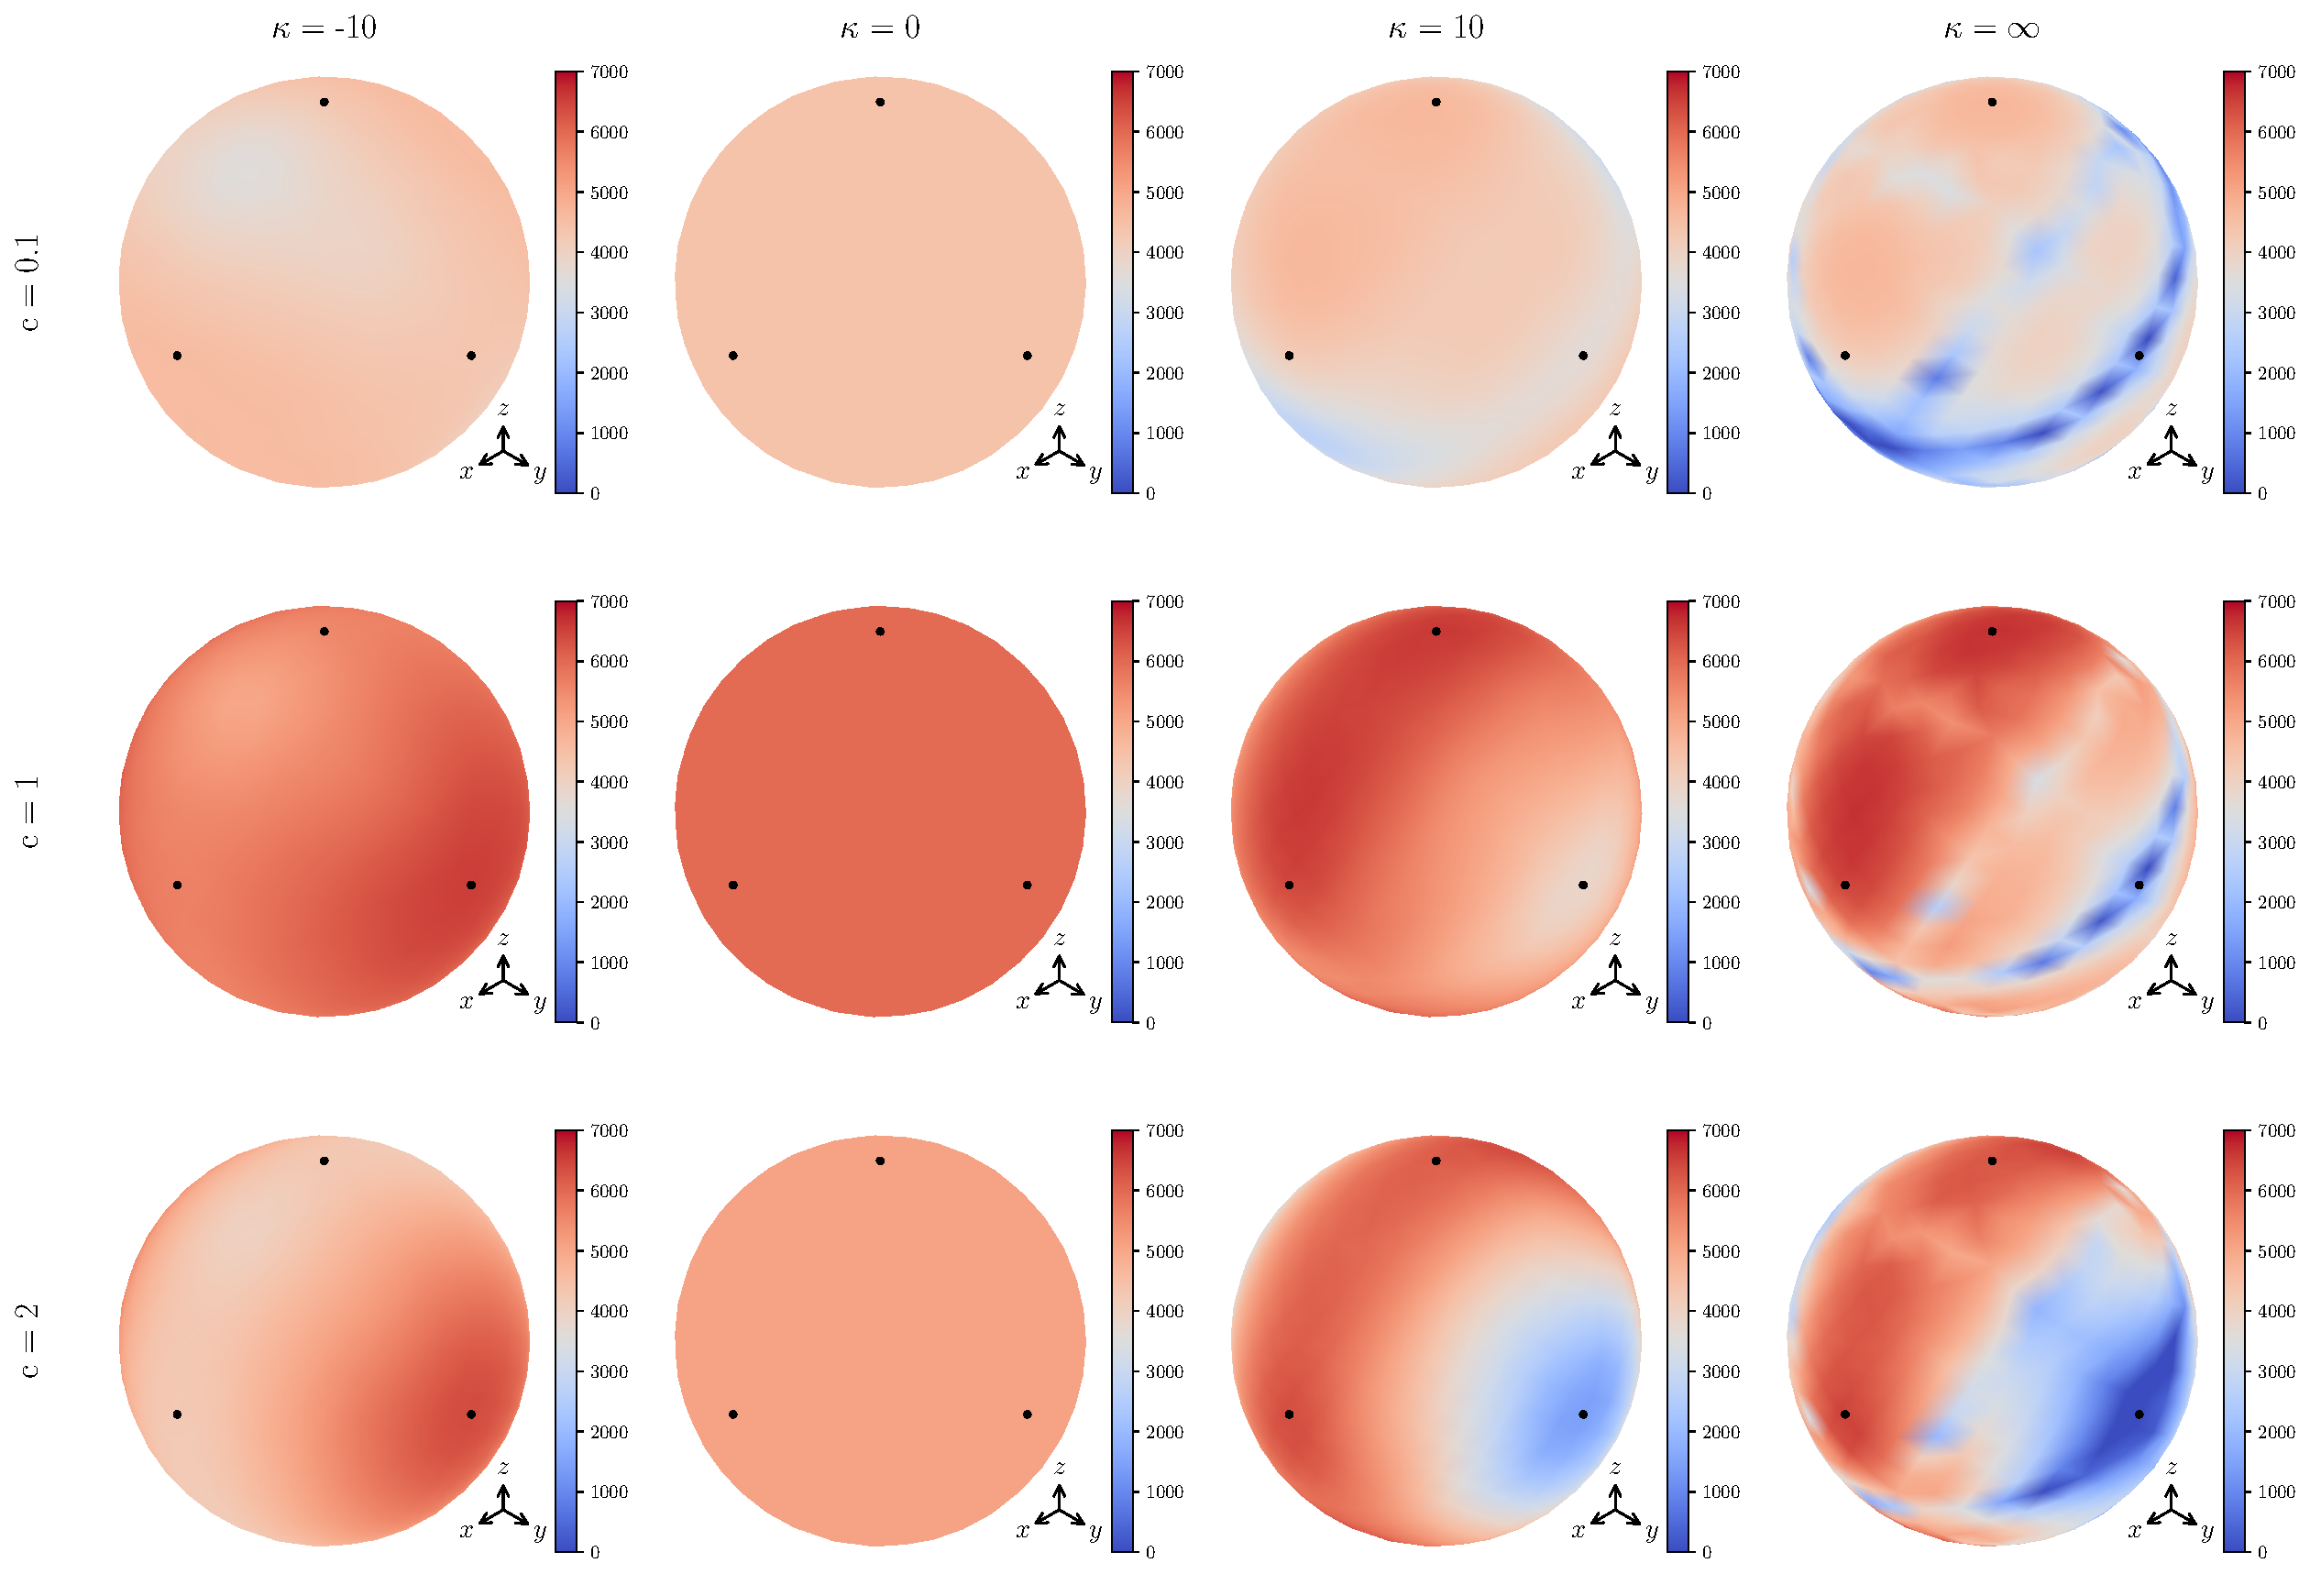
\includegraphics[width=0.9\textwidth, interpolate=true]{figs/likelihood-dist.pdf}\\
\end{center}
\end{frame}

\begin{frame}[label=sec-4]{Log-likelihood as a function of the fluorophore distribution ($\Theta$, $\Phi$, $\kappa$, $c$)}
\begin{center}
True orientation: $\Theta = 0, \Phi = 0, \kappa = 10, c = 1$\\
  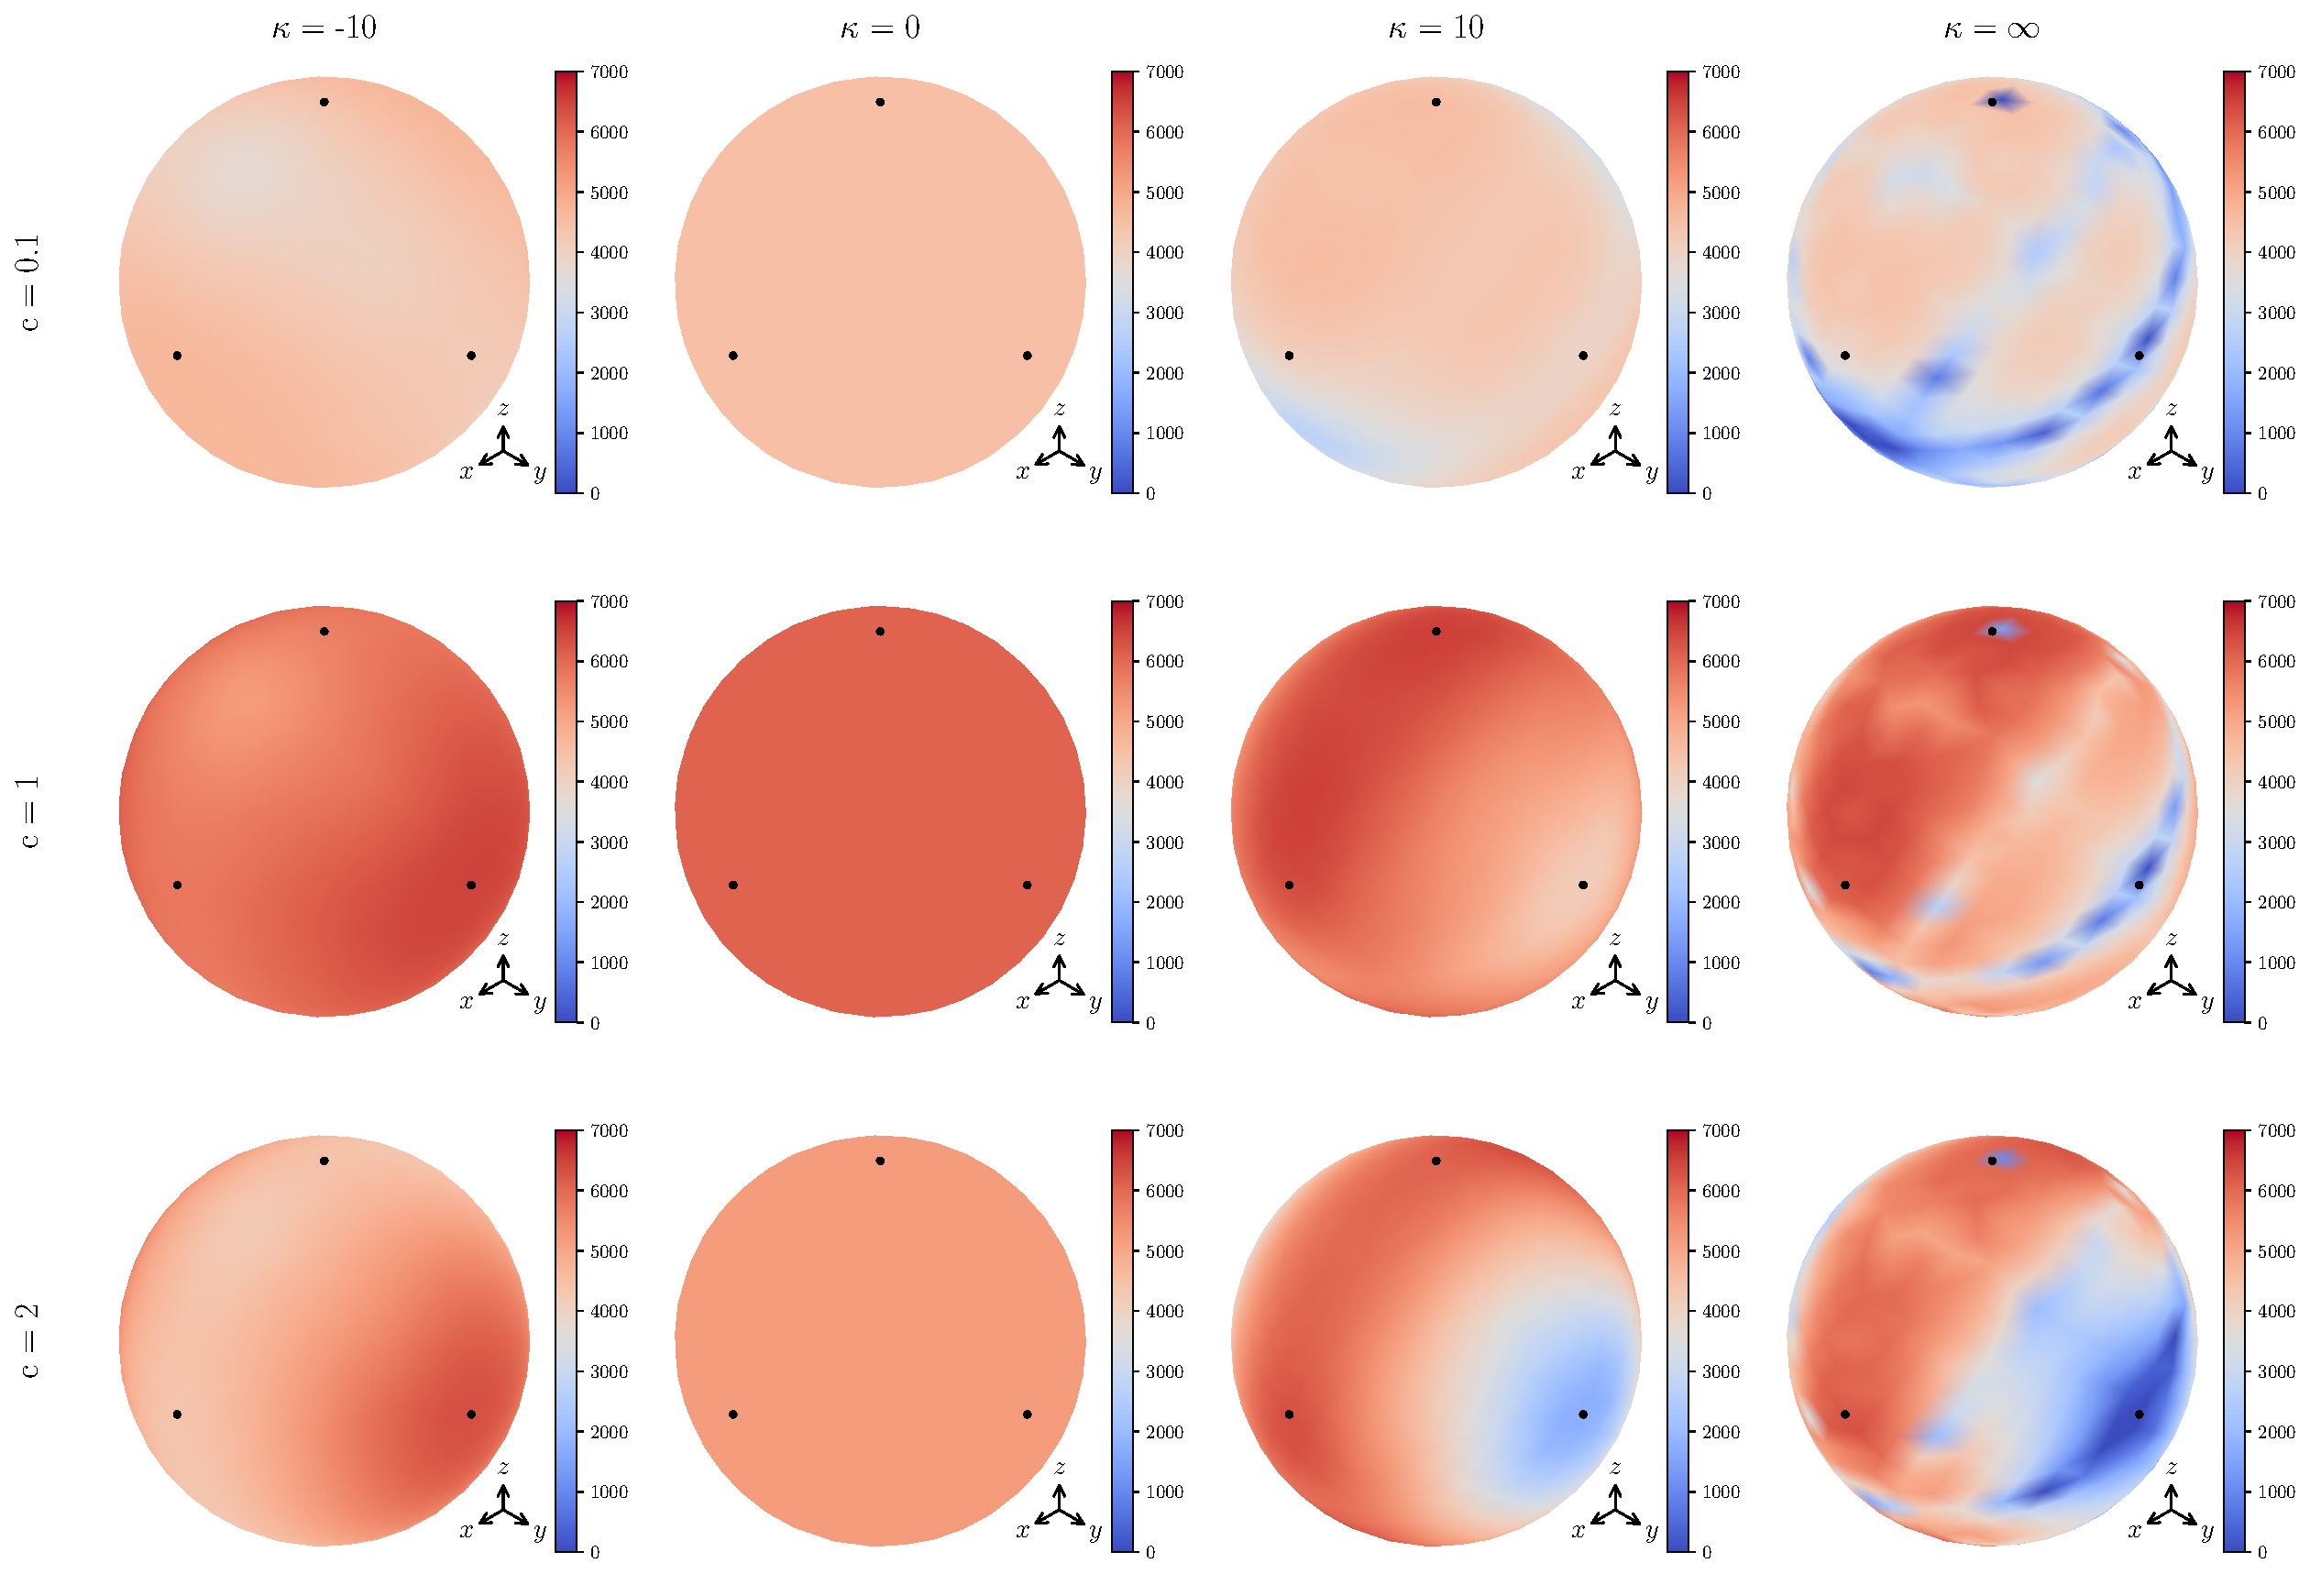
\includegraphics[width=0.9\textwidth, interpolate=true]{figs/likelihood-dist2.pdf}\\
\end{center}
\end{frame}
\begin{frame}[label=sec-5]{Discussion}
\begin{itemize}
\item $\Theta$ and $\Phi$ are bounded
\item $\kappa$ and $c$ are unbounded...estimate log($\kappa$) and log($c$) instead?
\end{itemize}
\end{frame}
% Emacs 25.3.1 (Org mode 8.2.10)
\end{document}